\chapter{Conclusiones y trabajo futuro}
\label{Capitulo_Conclusiones}
\label{Capitulo_6}
Este proyecto de tesis ha abordado el desafío de desarrollar un sistema de seguimiento móvil utilizando tecnología \acs{wifi}, centrándose en las técnicas de multilateración y perfilado, con el objetivo de estimar de manera precisa la ubicación de dispositivos móviles en entornos urbanos. A lo largo de esta investigación, se ha demostrado la viabilidad de implementar una solución tecnológica de bajo costo que puede ser integrada dentro del concepto de ciudades inteligentes, ofreciendo aplicaciones potenciales en \textit{Smart Parking} y el monitoreo del flujo peatonal y vehicular.
\section{Herramientas de Software Desarrolladas}
\label{herramientas_software}
Durante la elaboración de este trabajo, se desarrollaron múltiples herramientas de software para llevar a cabo las tareas de perfilado y multilateración, así como también el firmware de los ESP8266, script de la Raspberry PI y herramientas para gráficas.

A continuación se listarán los repositorios donde se contiene el código usado en este trabajo para cada una de dichas herramientas.
\begin{itemize}
    \item \href{https://pypi.org/project/easy-trilateration/#description}{\textbf{Easy-Trilateration}}: Se desarrolló una biblioteca de Python publicada en \textbf{PyPI} (Python Package Index), basada en otros trabajos \cite{madfolio}, para realizar multilateración con su correspondiente herramienta gráfica para facilitar su uso.

    \begin{figure}[th]
        \centering
        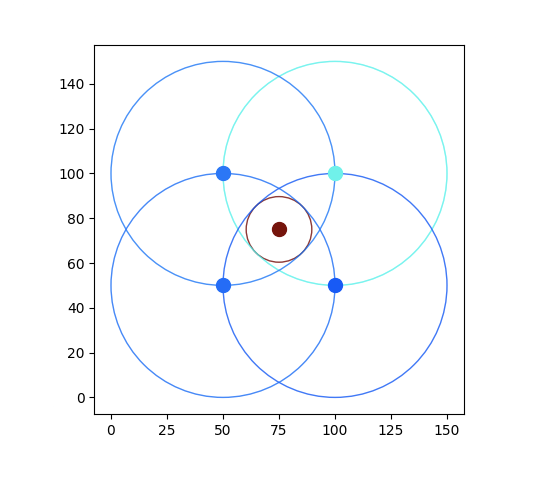
\includegraphics[width=0.8\textwidth]{Figuras/easy_trilateration.png}
        \captionsetup{margin=2cm}
        \caption[Herramienta gráfica de multilateración]{\href{https://github.com/agusalex/easy-trilateration}{\textbf{Herramienta gráfica de multilateración}}}
        \label{fig:libpython}
    \end{figure}

    \item \href{https://github.com/agusalex/rssi-filter-profiling}{\textbf{RSSI-Filter-Profiling}}: Herramienta que permite tomar múltiples capturas de perfilado, aplicar filtros como Kalman, mediana y promedio, realizar ajustes logarítmicos usando mínimos cuadrados y luego producir múltiples gráficas, incluyendo inversa y desviación estándar, comparando múltiples capturas de distintos dispositivos a la vez. También posee un combinador de gráficas, lo que permite tomar múltiples imágenes y convertirlas en una sola.

    \item \href{https://github.com/agusalex/ESP8266-sniffer-node}{\textbf{ESP8266-Sniffer-Node}}: Firmware para ESP8266 capaz de alternar entre el modo de captura de \textit{Probe Request} y el modo de subida de datos.

    \item \href{https://github.com/agusalex/ns3-rssi-trilateration}{\textbf{NS3-RSSI-Trilateration}}: Software que permite realizar perfilado y multilateración simulada usando NS3. Combina tanto \textbf{RSSI-Filter-Profiling} como \href{https://github.com/agusalex/easy-trilateration}{\textbf{Easy-Trilateration}} como submódulos de Git. Funciona aplicando un perfil de movilidad a un nodo, generando una captura simulada y luego graficando la reducción en la señal a medida que este se aleja, hallando los valores de \( A \) y \( N \). Posteriormente, permite simular un escenario de multilateración utilizando la herramienta mencionada. La idea de este software es ejecutar ambas simulaciones de manera sencilla.
\end{itemize}
\section{Hallazgos Principales}

Los experimentos realizados, tanto en entornos simulados como reales, han demostrado la capacidad de utilizar señales \acs{wifi} para localizar dispositivos móviles de manera efectiva. Este enfoque presenta una alternativa viable y de bajo costo a los sistemas basados en hardware especializado, ofreciendo una nueva herramienta para el análisis del comportamiento peatonal y vehicular en las ciudades.

A través de la investigación, se ha identificado la importancia de una disposición y configuración óptima de los nodos \textbf{Sniffer} para maximizar tanto la cobertura como la precisión de las estimaciones de ubicación. La interacción entre la disposición de los nodos y las características específicas del entorno urbano, como la cantidad de edificios, transeúntes y por sobre todo las interferencias electromagnéticas. Han demostrado ser un factores crítico en la eficacia de la localización.


\section{Limitaciones y Desafíos}

El proyecto enfrentó varias limitaciones técnicas y metodológicas. La precisión de las estimaciones de ubicación fue impactada por la interferencia inalámbrica y la variabilidad en la recepción de los dispositivos. Las limitaciones inherentes del hardware elegido y la infraestructura disponible para sostenerlo. Además, la práctica de la randomización de direcciones \acs{mac} en dispositivos modernos representa un desafío significativo para el seguimiento continuo de dispositivos a lo largo del tiempo.

\section{Recomendaciones para Futuras Investigaciones}
Para continuar avanzando en esta área, se considera importante:

\begin{itemize}
    \item Investigar en profundidad los efectos de la urbanización en la propagación de señales \acs{wifi} y desarrollar técnicas de corrección o compensación que mejoren la precisión en la estimación de la ubicación \cite{choi_2019_unsupervised}.
    \item Explorar utilizar \acs{gps}, para poder perfilar con precisión los nodos y así mejorar las estimaciones de ubicación obtenidas a través de \acs{wifi}.
    \item Desarrollar algoritmos de aprendizaje automático o alguna otra técnica para desenmascarar direcciones \acs{mac} que puedan identificar y seguir dispositivos a pesar de la randomización \acs{mac} \cite{baccichet2024mac}.
    \item Realizar experimentos adicionales en una variedad de entornos urbanos y con diferentes configuraciones de hardware para validar la robustez y adaptabilidad de las soluciones propuestas \cite{10.1007-978-3-030-11027}.
    \item Probar dichas técnicas con vehículos e instalaciones de \textit{Sniffers} sobre postes de luz para detectar vehículos estacionados\cite{yuansmartparking}.
    \item Explorar la posibilidad de detectar patrones de estacionamiento de automóviles, ciclistas que circulan por las calles y transeúntes en la vereda.
\end{itemize}

\section{Comentarios Finales}

La realización de esta tesis ha permitido explorar y expandir el conocimiento en el área de localización y seguimiento de dispositivos móviles en entornos urbanos, utilizando tecnología \acs{wifi} con micro-controladores de bajo costo. A pesar de enfrentar desafíos significativos, los resultados obtenidos proporcionan una base interesante para futuras investigaciones.

Mirando hacia adelante, es claro que la adopción de soluciones tecnológicas de tipo \textit{Smart Cities} jugará un papel fundamental en el diseño de las ciudades del futuro. Este trabajo contribuye a ese esfuerzo, sentando las bases para investigaciones futuras en el área de Smart Cities.